\documentclass[../main.tex]{subfiles}

\begin{document}

\Gls{spa} has significantly increased its popularity in the last decades. As a consequence, several image processing packages have arised. All of them chase similar ambitions: Obtain accurate high resolution maps in the least amount of time possible. Most of the state-of-the-art \gls{cryoem} image processing packages have converged into the same image processing pipeline. This pipeline follows a conventional structure, although it is somewhat malleable. The difference between packages lies on the algorithmic approach they use to accomplish individual tasks of the pipeline. Usually, each package is only proficient in a handful of steps. In fact, some packages do not implement the whole pipeline and rely on others to be able to process from beginning to end.

Traditional software packages in the context of \gls{spa} are Spider\cite{shaikh2008}, Imagic, Eman\cite{ludke2000}, Cistem\cite{grigorieff2018}, Relion\cite{scheres2021} and Xmipp\cite{sorzano2004}. In 2016 the introduction of Cryosparc\cite{cryosparc} was disruptive due to its significant performance improvements. Closely related to this, Scipion\cite{delarosa2016} is a platform that enables end users to easily interoperate between different image processing packages.

One of the recent leaps in the context of \gls{cryoem} has been the usage of hardware accelerators such as \glspl{gpu} to significantly reduce processing times. Although \glspl{gpu} are only well suited for highly parallelisable operations, in those cases, the computation time is reduced by several orders of magnitude. In fact, this has been one of the main factors leading to the recent growth of \gls{cryoem}.

Currently, all of the image processing suites are steering towards streaming image processing. This means that data is processed at the same time that it is acquired in the microscope. This allows to adjust acquisition parameters in real-time, optimising resource utilisation and improving the quality of the final results.

\subsection{Xmipp}
Xmipp is a image processing package aimed at obtaining 3D electron density maps of biological samples. It is developed at the \gls{bcu} group at the \gls{cnb}-\gls{csic} research centre. It was introduced at 1996, although it has suffered many major overhauls since then. Even though its primary focus is on \gls{spa}, it has diversified to many other microscopy techniques such as \gls{cryoet}\cite{sorzano2004}.

Currently it is on its third major version, which gets a minor version bump-up every 4 months. It has been mostly implemented in the C++ programming language, but it includes parts written in Python and Java. Xmipp offers methods for all steps in the \gls{spa} image processing pipeline, being proficient at movie alignment (Flexalign)\cite{strelak2021}, \gls{ctf} estimation, particle picking and 3D refinement.

Xmipp developers have ported many crucial programs to run on \gls{gpu} accelerators, significantly decreasing overall computation times. This has been achieved using \gls{cuda}, a \gls{gpu} computing platform commercialised by Nvidia Corporation.

\subsection{Scipion}
As mentioned earlier, Scipion does not implement any image processing algorithms. Instead, it provides a common scaffolding to integrate image processing packages though plugins. This enables end users to easily build \gls{spa} image processing workflows using the strengths of each processing package. Moreover, it provides methods to consensuate the outputs of multiple programs, further increasing the quality of the results. In fact, the benefits of Scipion have been extended to other domains such as Virtual Drug Screening\cite{scipion_chem} or \gls{cryoet}\cite{jimenezdelamorena2021}.

In the context of \gls{spa}, all widespread image processing tools have been integrated into Scipion. As shown in the Figure \ref{fig:3:scipion_statistics_type}, usage statistics prove that users do have different preferences for each step of the processing workflow. For instance, 3D classification is almost always done with Relion, whilst particle picking is primarily done though Xmipp. This proves the need for such a software, as manually inter-operating between packages is a very time consuming and error prone process. At the same time, being locked-in with a particular package leads to suboptimal results, as that particular package may waver in some steps.

\begin{figure}[htbp]
    \centering
    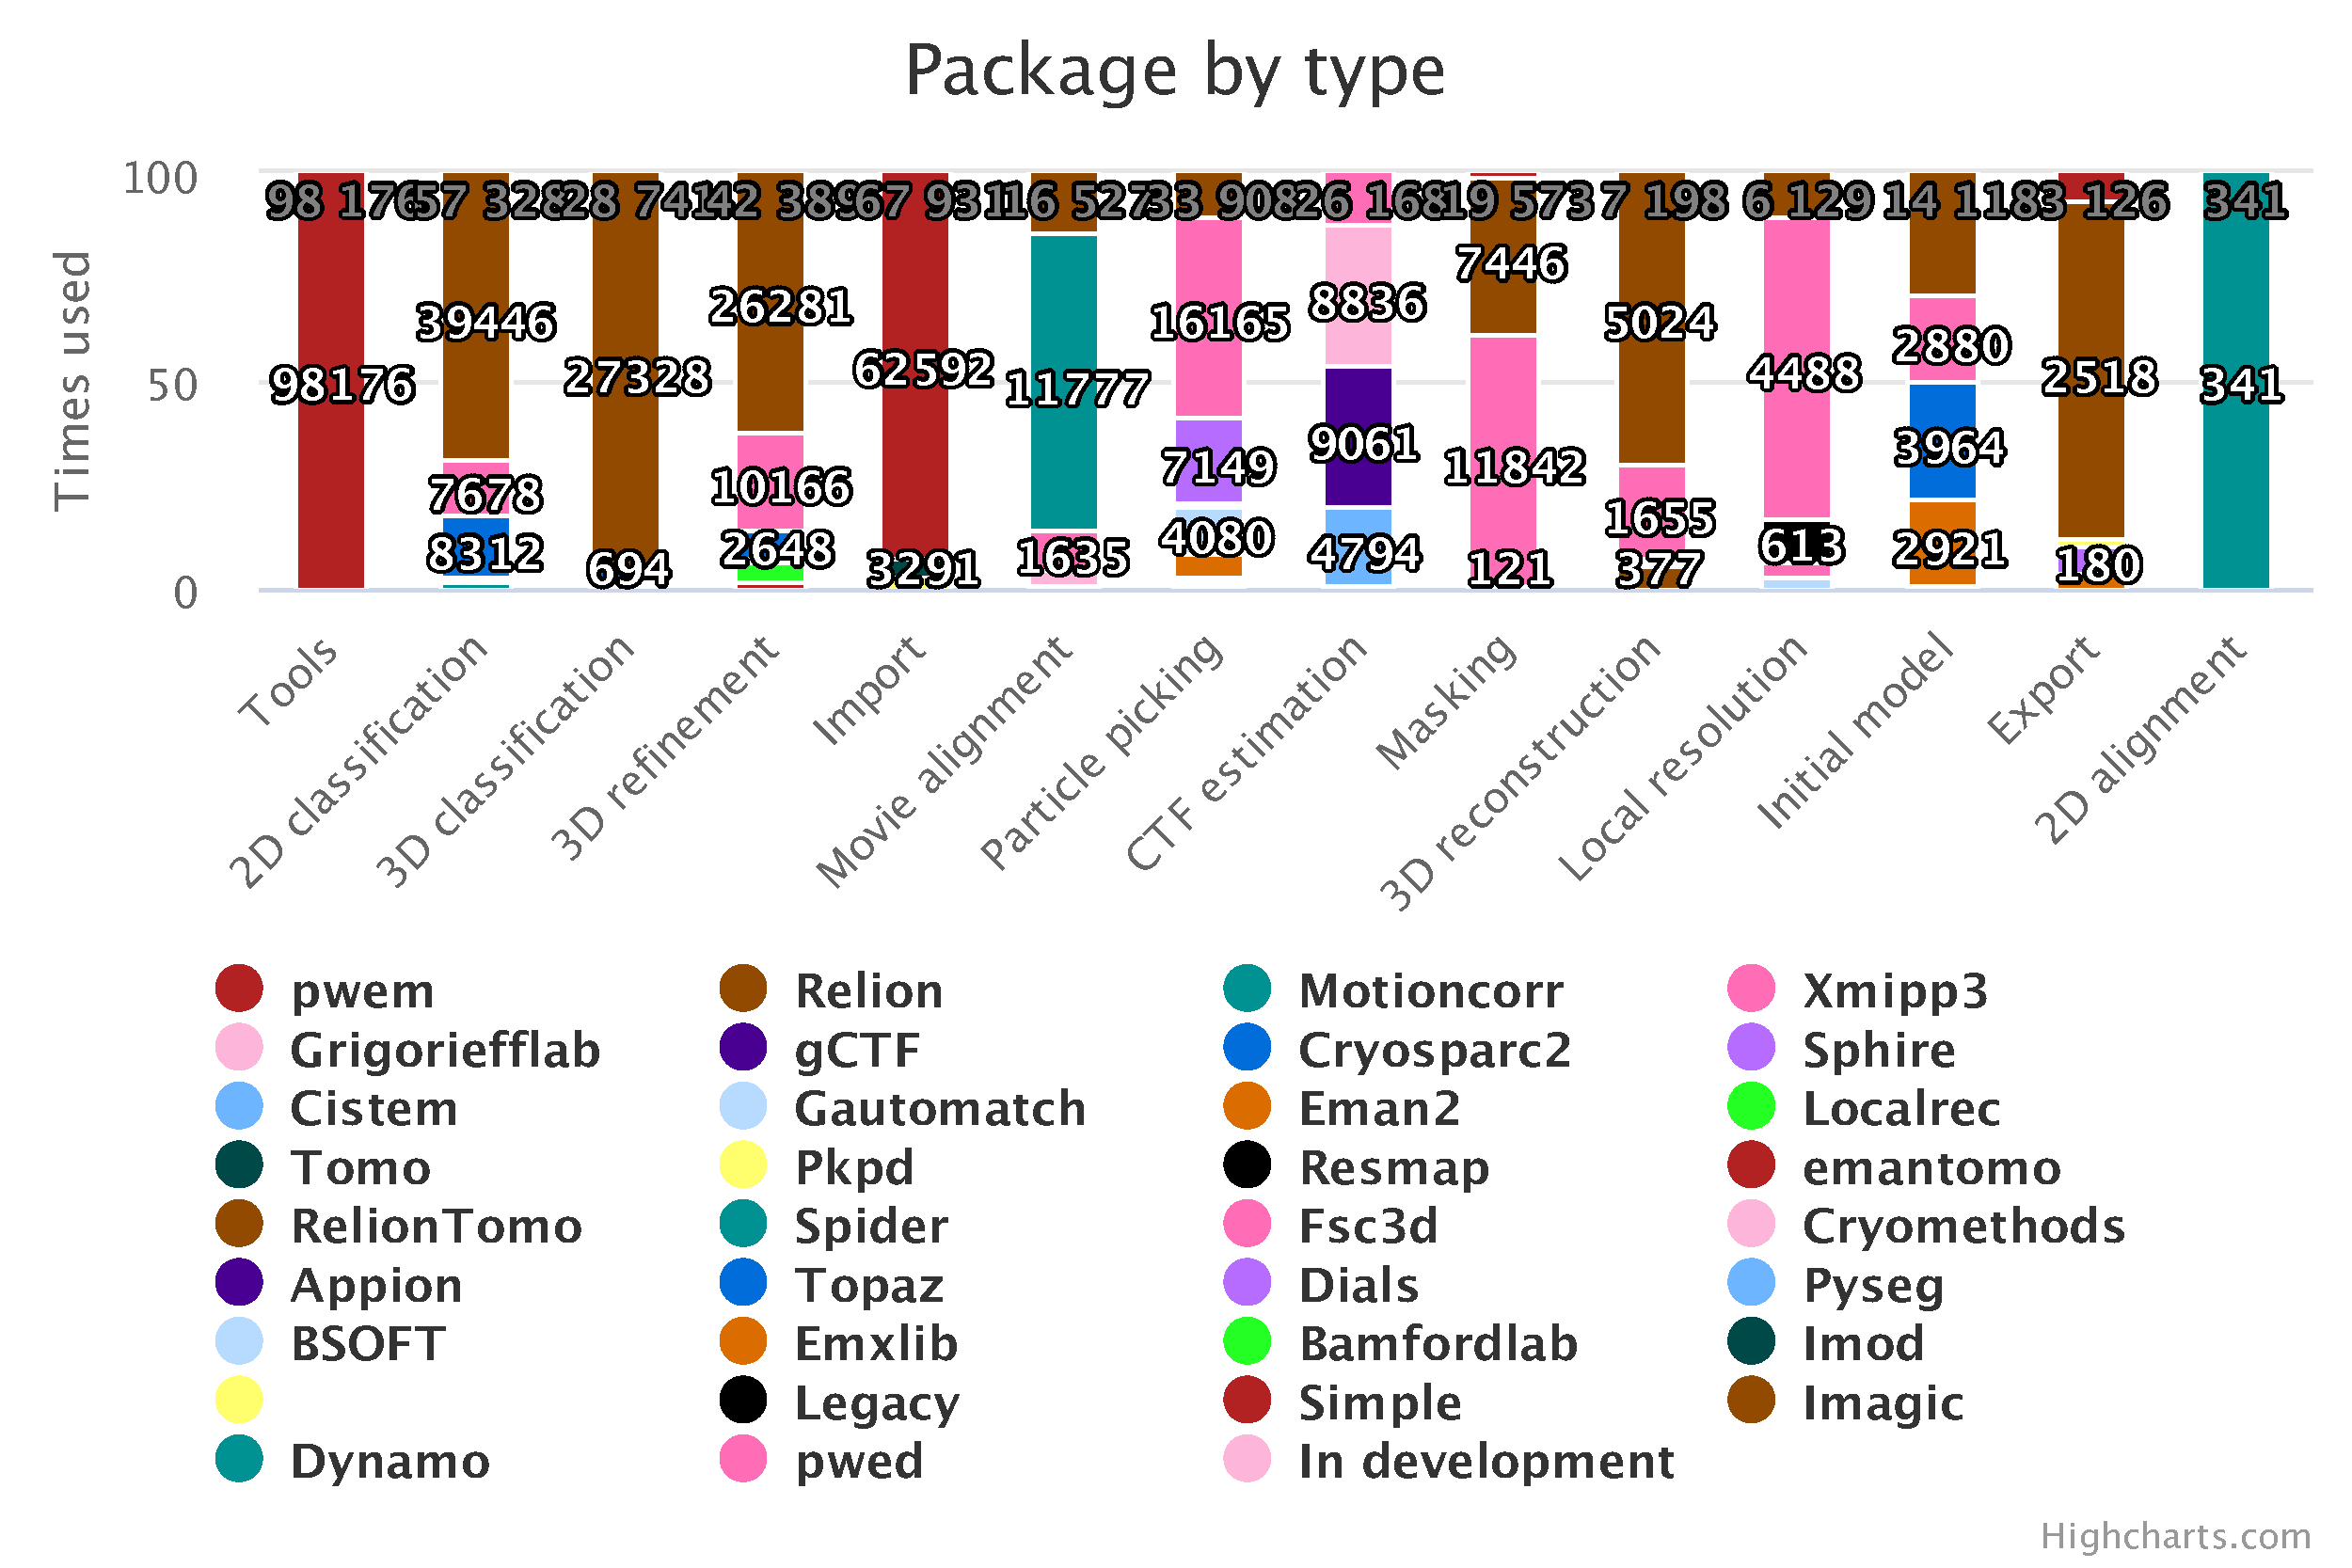
\includegraphics[width=\textwidth]{scipion_statistics/package-by-type}
    \caption{Scipion package usage statistics by type}
    \label{fig:3:scipion_statistics_type}
\end{figure}

Scipion is highly modular, as it can be extended with plugins. These plugins are usually related to the integration of a image processing suite, such as Relion or Cryosparc. A plugin provides a set of protocols, which can can be seen as a ``steps'' in the image processing workflow. Then, the user can easily build its own workflow, freely choosing the procedure used for each stage. What is more, the user may repeat the same step using different protocols and consensuate their outputs. Therefore, Scipion not only integrates alien algorithms, but it also provides some added value to the results.

Many of the current Scipion developments focus on implementing streaming workflows. All of the benefits stated earlier still apply to streaming workflows. Moreover, there is some innovation related to the automated control of the microscope from the image processing software. This control feedback loop enables microscope operation with little human intervention, significantly reducing costs.

\end{document}